\documentclass[11pt]{article}
\usepackage{geometry,marginnote} % Pour passer au format A4
\geometry{hmargin=1cm, vmargin=1cm} % 

% Page et encodage
\usepackage[T1]{fontenc} % Use 8-bit encoding that has 256 glyphs
\usepackage[english,french]{babel} % Français et anglais
\usepackage[utf8]{inputenc} 

\usepackage{lmodern}
\setlength\parindent{0pt}

% Graphiques
\usepackage{graphicx,float,grffile}
\usepackage{pst-eucl, pst-plot,units} 

% Maths et divers
\usepackage{amsmath,amsfonts,amssymb,amsthm,verbatim}
\usepackage{multicol,enumitem,url,eurosym,gensymb}
\DeclareUnicodeCharacter{20AC}{\euro}

% Sections
\usepackage{sectsty} % Allows customizing section commands
\allsectionsfont{\centering \normalfont\scshape}

% Tête et pied de page

\usepackage{fancyhdr} 
\pagestyle{fancyplain} 

\fancyhead{} % No page header
\fancyfoot{}

\renewcommand{\headrulewidth}{0pt} % Remove header underlines
\renewcommand{\footrulewidth}{0pt} % Remove footer underlines

\newcommand{\horrule}[1]{\rule{\linewidth}{#1}} % Create horizontal rule command with 1 argument of height

%----------------------------------------------------------------------------------------
%   Début du document
%----------------------------------------------------------------------------------------

\begin{document}


\textbf{Remarque} : \\
\textit{Attention, toutes les calculatrices ne donnent pas toujours les mêmes résultats} : $8 \div 2(2+2) =$ 16 (TI) ou 1 (Casio)

\begin{minipage}[t]{0.5\textwidth}
  \begin{figure}[H]
        \centering
        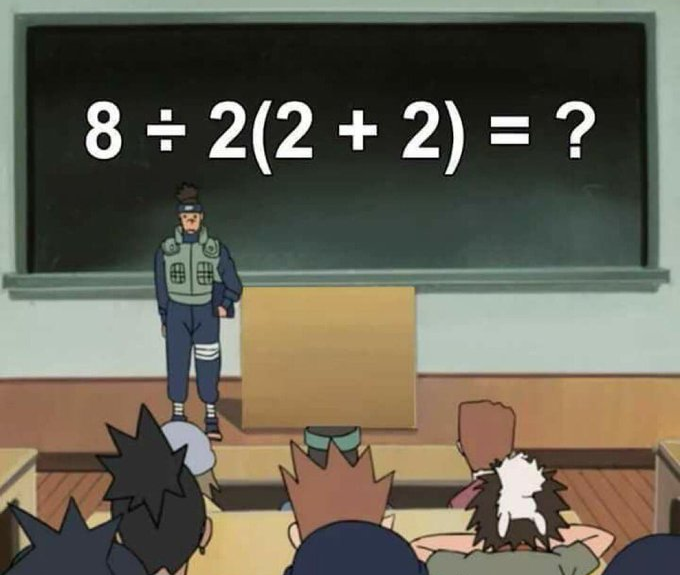
\includegraphics[width=0.7\linewidth]{5x1-calculer-et-rediger-des-calculs/naruto.png}
  \end{figure}
\end{minipage}
\begin{minipage}[t]{0.5\textwidth}
  \begin{figure}[H]
        \centering
        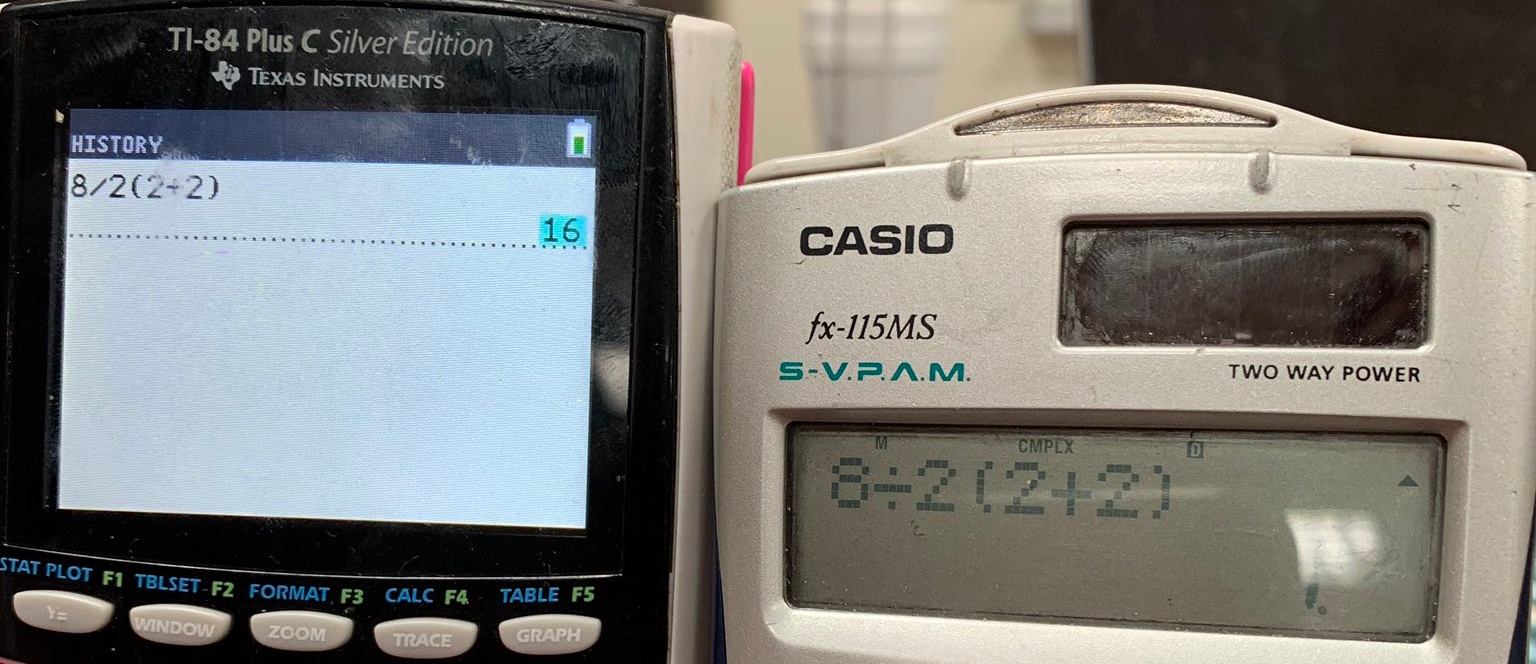
\includegraphics[width=\linewidth]{5x1-calculer-et-rediger-des-calculs/calc.png}
  \end{figure}
... cela veut dire que le calcul est mal écrit ...
\end{minipage}


\section*{3 - Calculer astucieusement}

Il est possible d'ête \textbf{malin} quand on fait des calculs. Il faut faire attention à bien respecter les règles de calculs...

\begin{minipage}[t]{0.33\textwidth}
\begin{align*}
25 + 7 + 75 &= 100 + 7  \\
            &= 107
\end{align*}

\end{minipage}
\begin{minipage}[t]{0.33\textwidth}

\begin{align*}
102 \times 6 &= 600 + 2 \times 6 \\
             &= 600 + 12 \\
             &= 612
\end{align*}

\end{minipage}
\begin{minipage}[t]{0.33\textwidth}

\begin{align*}
5 \times 7 \times 2 &= 10 \times 7 \\
                    &= 70
\end{align*}
\end{minipage}

\vspace{0.5cm}\horrule{1px}\vspace{0.5cm}


\textbf{Remarque} : \\
\textit{Attention, toutes les calculatrices ne donnent pas toujours les mêmes résultats} : $8 \div 2(2+2) =$ 16 (TI) ou 1 (Casio)

\begin{minipage}[t]{0.5\textwidth}
  \begin{figure}[H]
        \centering
        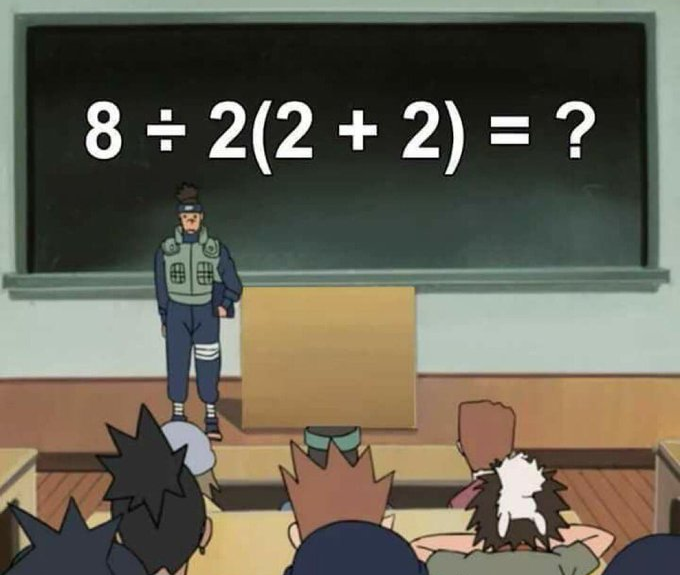
\includegraphics[width=0.7\linewidth]{5x1-calculer-et-rediger-des-calculs/naruto.png}
  \end{figure}
\end{minipage}
\begin{minipage}[t]{0.5\textwidth}
  \begin{figure}[H]
        \centering
        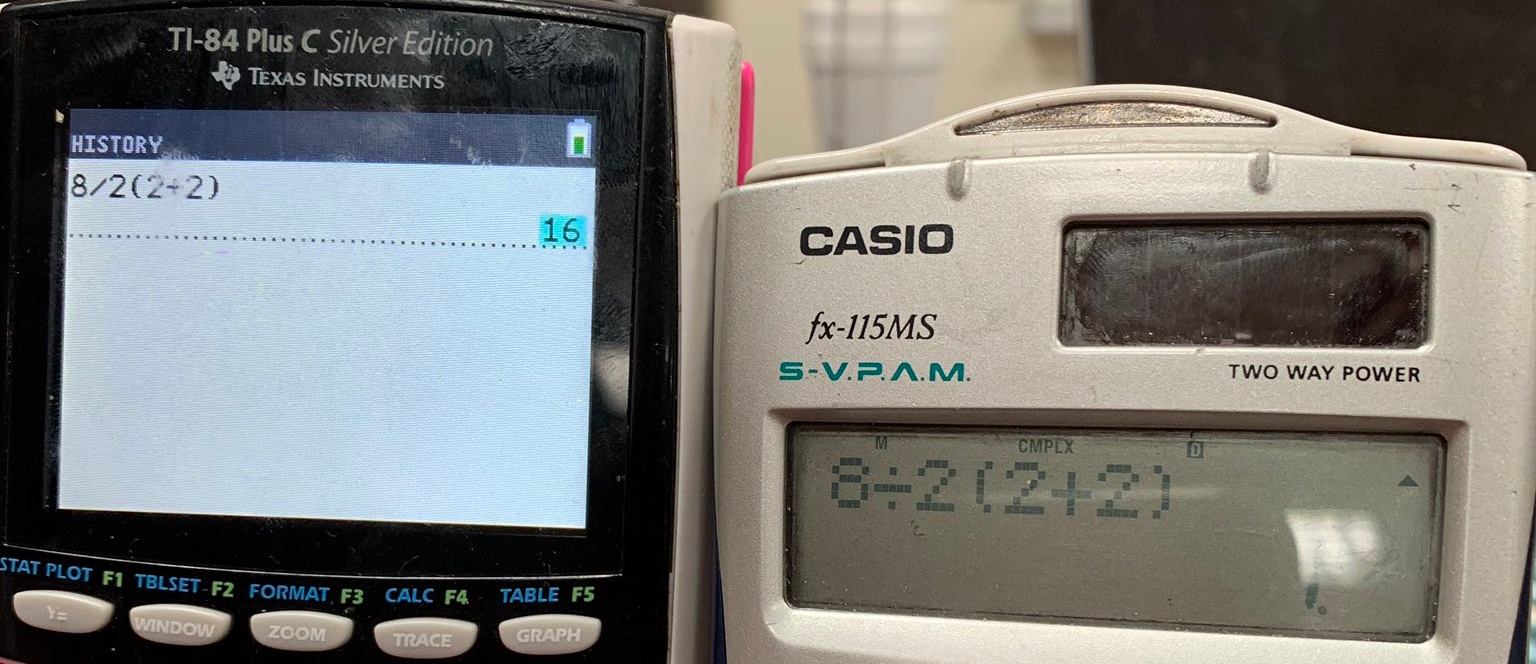
\includegraphics[width=\linewidth]{5x1-calculer-et-rediger-des-calculs/calc.png}
  \end{figure}
... cela veut dire que le calcul est mal écrit ...
\end{minipage}


\section*{3 - Calculer astucieusement}

Il est possible d'ête \textbf{malin} quand on fait des calculs. Il faut faire attention à bien respecter les règles de calculs...

\begin{minipage}[t]{0.33\textwidth}
\begin{align*}
25 + 7 + 75 &= 100 + 7  \\
            &= 107
\end{align*}

\end{minipage}
\begin{minipage}[t]{0.33\textwidth}

\begin{align*}
102 \times 6 &= 600 + 2 \times 6 \\
             &= 600 + 12 \\
             &= 612
\end{align*}

\end{minipage}
\begin{minipage}[t]{0.33\textwidth}

\begin{align*}
5 \times 7 \times 2 &= 10 \times 7 \\
                    &= 70
\end{align*}
\end{minipage}

\newpage

\textbf{Remarque} : \\
\textit{Attention, toutes les calculatrices ne donnent pas toujours les mêmes résultats} : $8 \div 2(2+2) =$ 16 (TI) ou 1 (Casio)

\begin{minipage}[t]{0.5\textwidth}
  \begin{figure}[H]
        \centering
        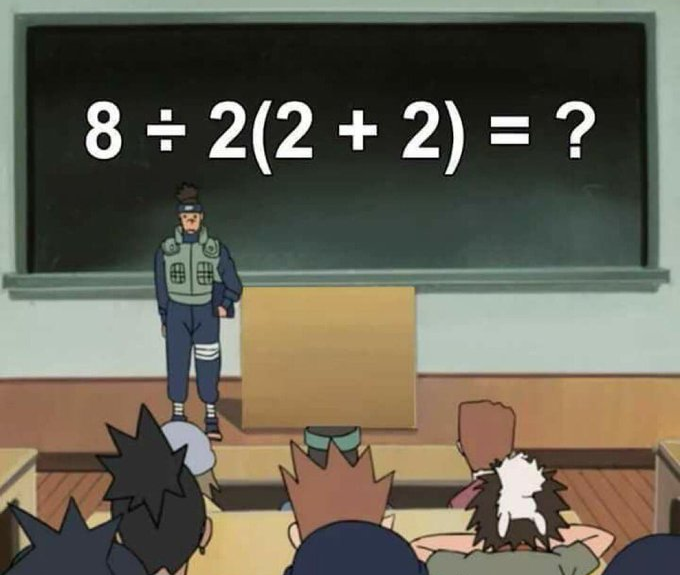
\includegraphics[width=0.7\linewidth]{5x1-calculer-et-rediger-des-calculs/naruto.png}
  \end{figure}
\end{minipage}
\begin{minipage}[t]{0.5\textwidth}
  \begin{figure}[H]
        \centering
        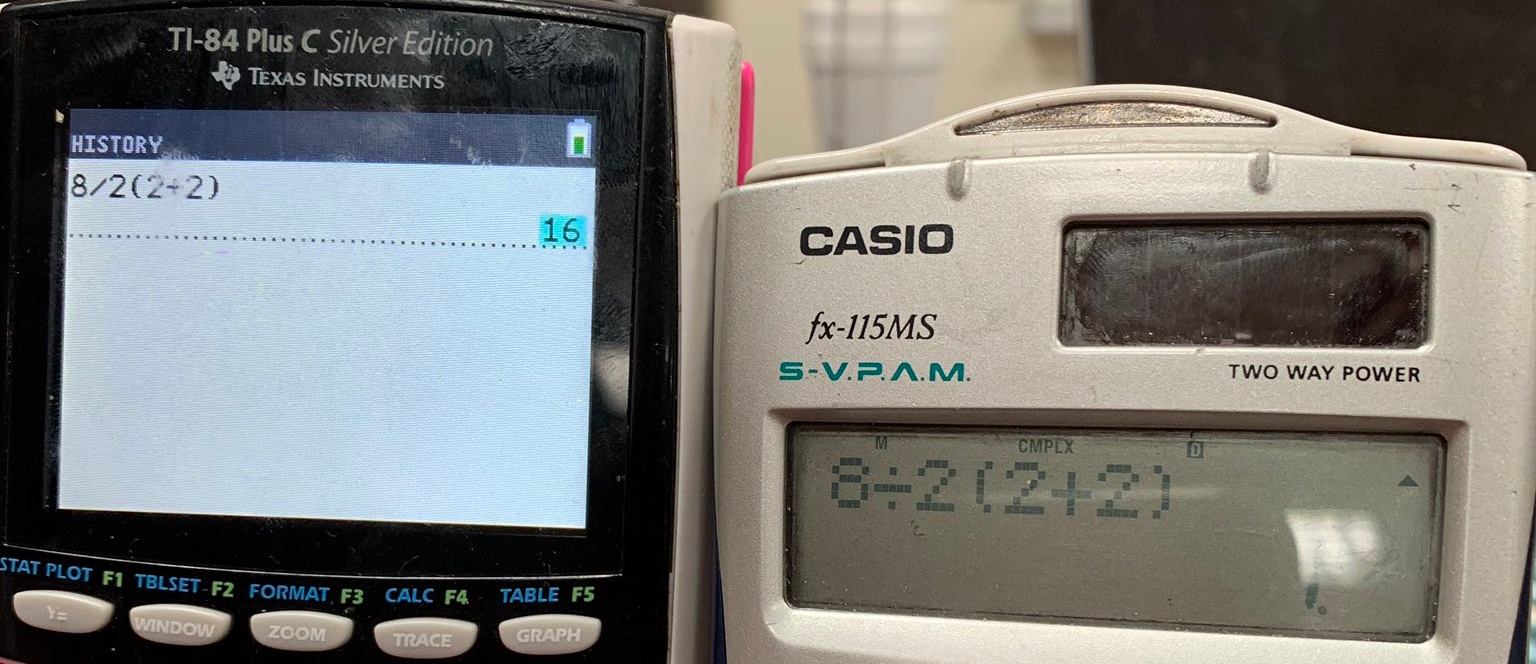
\includegraphics[width=\linewidth]{5x1-calculer-et-rediger-des-calculs/calc.png}
  \end{figure}
... cela veut dire que le calcul est mal écrit ...
\end{minipage}


\section*{3 - Calculer astucieusement}

Il est possible d'ête \textbf{malin} quand on fait des calculs. Il faut faire attention à bien respecter les règles de calculs...

\begin{minipage}[t]{0.33\textwidth}
\begin{align*}
25 + 7 + 75 &= 100 + 7  \\
            &= 107
\end{align*}

\end{minipage}
\begin{minipage}[t]{0.33\textwidth}

\begin{align*}
102 \times 6 &= 600 + 2 \times 6 \\
             &= 600 + 12 \\
             &= 612
\end{align*}

\end{minipage}
\begin{minipage}[t]{0.33\textwidth}

\begin{align*}
5 \times 7 \times 2 &= 10 \times 7 \\
                    &= 70
\end{align*}
\end{minipage}

\vspace{0.5cm}\horrule{1px}\vspace{0.5cm}

\textbf{Remarque} : \\
\textit{Attention, toutes les calculatrices ne donnent pas toujours les mêmes résultats} : $8 \div 2(2+2) =$ 16 (TI) ou 1 (Casio)

\begin{minipage}[t]{0.5\textwidth}
  \begin{figure}[H]
        \centering
        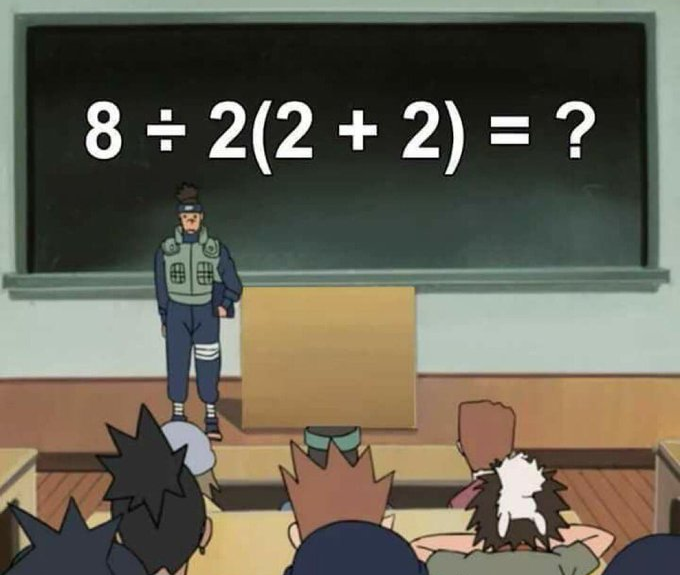
\includegraphics[width=0.7\linewidth]{5x1-calculer-et-rediger-des-calculs/naruto.png}
  \end{figure}
\end{minipage}
\begin{minipage}[t]{0.5\textwidth}
  \begin{figure}[H]
        \centering
        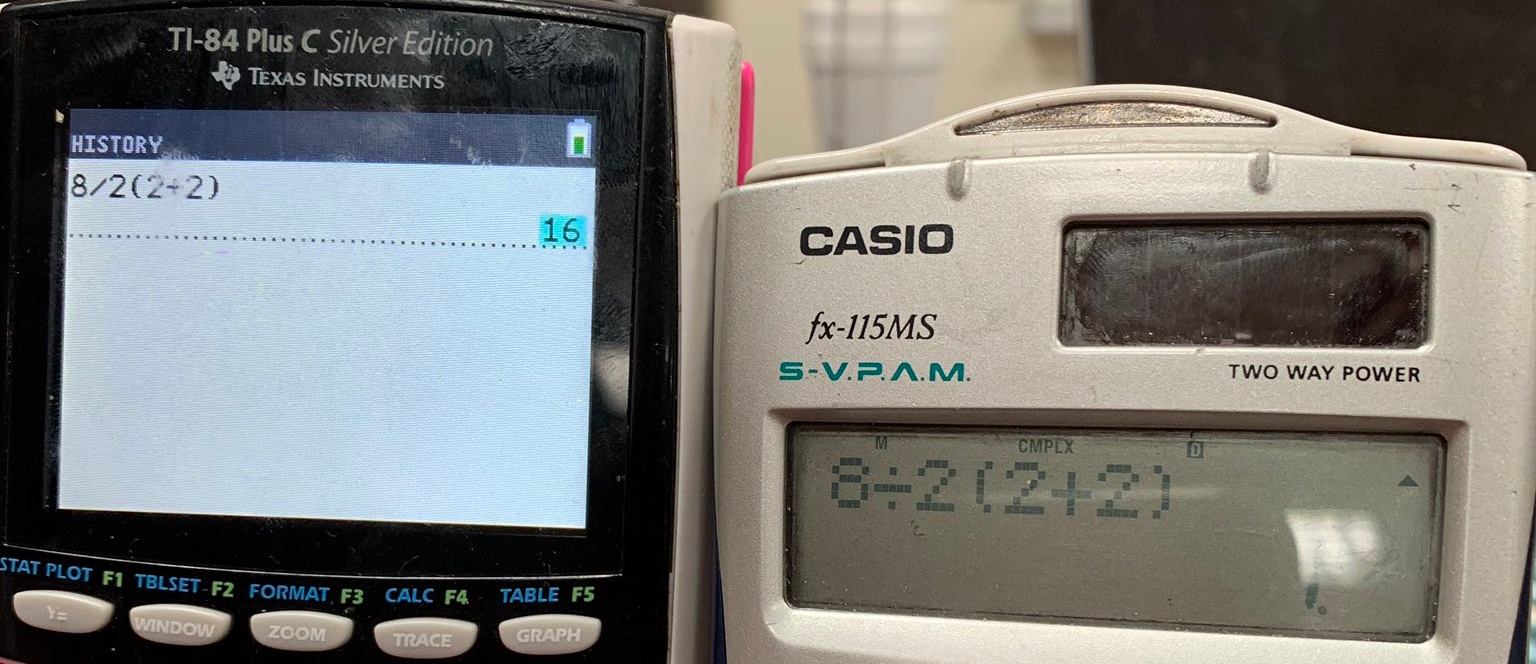
\includegraphics[width=\linewidth]{5x1-calculer-et-rediger-des-calculs/calc.png}
  \end{figure}
... cela veut dire que le calcul est mal écrit ...
\end{minipage}


\section*{3 - Calculer astucieusement}

Il est possible d'ête \textbf{malin} quand on fait des calculs. Il faut faire attention à bien respecter les règles de calculs...

\begin{minipage}[t]{0.33\textwidth}
\begin{align*}
25 + 7 + 75 &= 100 + 7  \\
            &= 107
\end{align*}

\end{minipage}
\begin{minipage}[t]{0.33\textwidth}

\begin{align*}
102 \times 6 &= 600 + 2 \times 6 \\
             &= 600 + 12 \\
             &= 612
\end{align*}

\end{minipage}
\begin{minipage}[t]{0.33\textwidth}

\begin{align*}
5 \times 7 \times 2 &= 10 \times 7 \\
                    &= 70
\end{align*}
\end{minipage}

\newpage

\section*{5 - Répondre à un problème}

Parfois les exercices de type problème ne donnent pas directement le calcul à faire. Il faut d'abord créer l'expression. On appelle cette compétence \textbf{Modéliser}.\\

\textsc{\textbf{Exercice} : Pour la rentrée, j'achète une règle à 1,20€, trois crayons à papiers à 1,10€ l'unité et deux 4-couleurs à 2,50€.} \newline
\textsc{Calculer le prix à payer en caisse ?}\\

\textsc{\textbf{Correction} :}\\

Calcul du prix à payer :
\begin{align*}
1,20 + 3 \times 1,10 + 2 \times 2,50 &= 1,20 + 3,30 + 5 \\
                                     &= 9,5
\end{align*}

Le prix a payer en caisse est 9,50€.

\vspace{0.5cm}\horrule{1px}\vspace{0.5cm}

Parfois les exercices de type problème ne donnent pas directement le calcul à faire. Il faut d'abord créer l'expression. On appelle cette compétence \textbf{Modéliser}.\\

\textsc{\textbf{Exercice} : Pour la rentrée, j'achète une règle à 1,20€, trois crayons à papiers à 1,10€ l'unité et deux 4-couleurs à 2,50€.} \newline
\textsc{Calculer le prix à payer en caisse ?}\\

\textsc{\textbf{Correction} :}\\

Calcul du prix à payer :
\begin{align*}
1,20 + 3 \times 1,10 + 2 \times 2,50 &= 1,20 + 3,30 + 5 \\
                                     &= 9,5
\end{align*}

Le prix a payer en caisse est 9,50€.

\vspace{0.5cm}\horrule{1px}\vspace{0.5cm}

Parfois les exercices de type problème ne donnent pas directement le calcul à faire. Il faut d'abord créer l'expression. On appelle cette compétence \textbf{Modéliser}.\\

\textsc{\textbf{Exercice} : Pour la rentrée, j'achète une règle à 1,20€, trois crayons à papiers à 1,10€ l'unité et deux 4-couleurs à 2,50€.} \newline
\textsc{Calculer le prix à payer en caisse ?}\\

\textsc{\textbf{Correction} :}\\

Calcul du prix à payer :
\begin{align*}
1,20 + 3 \times 1,10 + 2 \times 2,50 &= 1,20 + 3,30 + 5 \\
                                     &= 9,5
\end{align*}

Le prix a payer en caisse est 9,50€.

\newpage

\section*{5 - Répondre à un problème}

Parfois les exercices de type problème ne donnent pas directement le calcul à faire. Il faut d'abord créer l'expression. On appelle cette compétence \textbf{Modéliser}.\\

\textsc{\textbf{Exercice} : Pour la rentrée, j'achète une règle à 1,20€, trois crayons à papiers à 1,10€ l'unité et deux 4-couleurs à 2,50€.} \newline
\textsc{Calculer le prix à payer en caisse ?}\\

\textsc{\textbf{Correction} :}\\

Calcul du prix à payer :
\begin{align*}
1,20 + 3 \times 1,10 + 2 \times 2,50 &= 1,20 + 3,30 + 5 \\
                                     &= 9,5
\end{align*}

Le prix a payer en caisse est 9,50€.

\vspace{0.5cm}\horrule{1px}\vspace{0.5cm}


Parfois les exercices de type problème ne donnent pas directement le calcul à faire. Il faut d'abord créer l'expression. On appelle cette compétence \textbf{Modéliser}.\\

\textsc{\textbf{Exercice} : Pour la rentrée, j'achète une règle à 1,20€, trois crayons à papiers à 1,10€ l'unité et deux 4-couleurs à 2,50€.} \newline
\textsc{Calculer le prix à payer en caisse ?}\\

\textsc{\textbf{Correction} :}\\

Calcul du prix à payer :
\begin{align*}
1,20 + 3 \times 1,10 + 2 \times 2,50 &= 1,20 + 3,30 + 5 \\
                                     &= 9,5
\end{align*}

Le prix a payer en caisse est 9,50€.

\vspace{0.5cm}\horrule{1px}\vspace{0.5cm}

Parfois les exercices de type problème ne donnent pas directement le calcul à faire. Il faut d'abord créer l'expression. On appelle cette compétence \textbf{Modéliser}.\\

\textsc{\textbf{Exercice} : Pour la rentrée, j'achète une règle à 1,20€, trois crayons à papiers à 1,10€ l'unité et deux 4-couleurs à 2,50€.} \newline
\textsc{Calculer le prix à payer en caisse ?}\\

\textsc{\textbf{Correction} :}\\

Calcul du prix à payer :
\begin{align*}
1,20 + 3 \times 1,10 + 2 \times 2,50 &= 1,20 + 3,30 + 5 \\
                                     &= 9,5
\end{align*}

Le prix a payer en caisse est 9,50€.

\newpage

\section*{6 - Répondre à un programme de calcul}

Cet exercice particulier mérite sa place dans le cours. C'est un programme de calcul. On fait des calculs les uns à la suite des autres. Créer l'expression est un peu plus dur et demande parfois de rajouter des parenthèses. Il faut aussi connaitre un peu de vocabulaire en français ! Retrancher, Soustraire Ajouter, Additionner, Prendre le double... \\

\textbf{Exercice} : 

\begin{center}\fbox{\begin{minipage}{0.4\textwidth}
  {\fontfamily{lmtt}\selectfont 
    \begin{itemize}
      \item Prendre le nombre de départ.
      \item Ajouter 10.
      \item multiplier par 4.
      \item Retrancher 40.
    \end{itemize}
  }
\end{minipage}}\end{center}

\textsc{Faire le programme de calcul avec : 0, 2, 100.} \\

\textbf{Correction} :

\begin{minipage}{0.3\textwidth}

\begin{align*}
& 0 \\
& 0 + 10 = 10 \\
& 10 \times 4 = 40\\
& 40 - 40 = 0
\end{align*}

\end{minipage}\begin{minipage}{0.3\textwidth}

\begin{align*}
& 2 \\
& 2 + 10 = 12 \\
& 12 \times 4 = 48\\
& 48 - 40 = 8
\end{align*}

\end{minipage}\begin{minipage}{0.3\textwidth}

\begin{align*}
& 100 \\
& 100 + 10 = 110 \\
& 110 \times 4 = 440\\
& 440 - 40 = 400
\end{align*}

\end{minipage}

\vspace{1.5cm}\horrule{1px}\vspace{1.5cm}

Cet exercice particulier mérite sa place dans le cours. C'est un programme de calcul. On fait des calculs les uns à la suite des autres. Créer l'expression est un peu plus dur et demande parfois de rajouter des parenthèses. Il faut aussi connaitre un peu de vocabulaire en français ! Retrancher, Soustraire Ajouter, Additionner, Prendre le double... \\

\textbf{Exercice} : 

\begin{center}\fbox{\begin{minipage}{0.4\textwidth}
  {\fontfamily{lmtt}\selectfont 
    \begin{itemize}
      \item Prendre le nombre de départ.
      \item Ajouter 10.
      \item multiplier par 4.
      \item Retrancher 40.
    \end{itemize}
  }
\end{minipage}}\end{center}

\textsc{Faire le programme de calcul avec : 0, 2, 100.} \\

\textbf{Correction} :

\begin{minipage}{0.3\textwidth}

\begin{align*}
& 0 \\
& 0 + 10 = 10 \\
& 10 \times 4 = 40\\
& 40 - 40 = 0
\end{align*}

\end{minipage}\begin{minipage}{0.3\textwidth}

\begin{align*}
& 2 \\
& 2 + 10 = 12 \\
& 12 \times 4 = 48\\
& 48 - 40 = 8
\end{align*}

\end{minipage}\begin{minipage}{0.3\textwidth}

\begin{align*}
& 100 \\
& 100 + 10 = 110 \\
& 110 \times 4 = 440\\
& 440 - 40 = 400
\end{align*}

\end{minipage}
\newpage

\section*{6 - Répondre à un programme de calcul}

Cet exercice particulier mérite sa place dans le cours. C'est un programme de calcul. On fait des calculs les uns à la suite des autres. Créer l'expression est un peu plus dur et demande parfois de rajouter des parenthèses. Il faut aussi connaitre un peu de vocabulaire en français ! Retrancher, Soustraire Ajouter, Additionner, Prendre le double... \\

\textbf{Exercice} : 

\begin{center}\fbox{\begin{minipage}{0.4\textwidth}
  {\fontfamily{lmtt}\selectfont 
    \begin{itemize}
      \item Prendre le nombre de départ.
      \item Ajouter 10.
      \item multiplier par 4.
      \item Retrancher 40.
    \end{itemize}
  }
\end{minipage}}\end{center}

\textsc{Faire le programme de calcul avec : 0, 2, 100.} \\

\textbf{Correction} :

\begin{minipage}{0.3\textwidth}

\begin{align*}
& 0 \\
& 0 + 10 = 10 \\
& 10 \times 4 = 40\\
& 40 - 40 = 0
\end{align*}

\end{minipage}\begin{minipage}{0.3\textwidth}

\begin{align*}
& 2 \\
& 2 + 10 = 12 \\
& 12 \times 4 = 48\\
& 48 - 40 = 8
\end{align*}

\end{minipage}\begin{minipage}{0.3\textwidth}

\begin{align*}
& 100 \\
& 100 + 10 = 110 \\
& 110 \times 4 = 440\\
& 440 - 40 = 400
\end{align*}

\end{minipage}

\vspace{1.5cm}\horrule{1px}\vspace{1.5cm}

Cet exercice particulier mérite sa place dans le cours. C'est un programme de calcul. On fait des calculs les uns à la suite des autres. Créer l'expression est un peu plus dur et demande parfois de rajouter des parenthèses. Il faut aussi connaitre un peu de vocabulaire en français ! Retrancher, Soustraire Ajouter, Additionner, Prendre le double... \\

\textbf{Exercice} : 

\begin{center}\fbox{\begin{minipage}{0.4\textwidth}
  {\fontfamily{lmtt}\selectfont 
    \begin{itemize}
      \item Prendre le nombre de départ.
      \item Ajouter 10.
      \item multiplier par 4.
      \item Retrancher 40.
    \end{itemize}
  }
\end{minipage}}\end{center}

\textsc{Faire le programme de calcul avec : 0, 2, 100.} \\

\textbf{Correction} :

\begin{minipage}{0.3\textwidth}

\begin{align*}
& 0 \\
& 0 + 10 = 10 \\
& 10 \times 4 = 40\\
& 40 - 40 = 0
\end{align*}

\end{minipage}\begin{minipage}{0.3\textwidth}

\begin{align*}
& 2 \\
& 2 + 10 = 12 \\
& 12 \times 4 = 48\\
& 48 - 40 = 8
\end{align*}

\end{minipage}\begin{minipage}{0.3\textwidth}

\begin{align*}
& 100 \\
& 100 + 10 = 110 \\
& 110 \times 4 = 440\\
& 440 - 40 = 400
\end{align*}

\end{minipage}

\end{document}
